% XeLaTeX can use any Mac OS X font. See the setromanfont command below.
% Input to XeLaTeX is full Unicode, so Unicode characters can be typed directly into the source.

% The next lines tell TeXShop to typeset with xelatex, and to open and save the source with Unicode encoding.

%!TEX TS-program = xelatex
%!TEX encoding = UTF-8 Unicode

\documentclass[14pt]{extreport}
\usepackage{geometry}                % See geometry.pdf to learn the layout options. There are lots.
\geometry{letterpaper}                   % ... or a4paper or a5paper or ... 
%\geometry{landscape}                % Activate for for rotated page geometry
%\usepackage[parfill]{parskip}    % Activate to begin paragraphs with an empty line rather than an indent
\usepackage{graphicx}
\usepackage{amssymb}

% Will Robertson's fontspec.sty can be used to simplify font choices.
% To experiment, open /Applications/Font Book to examine the fonts provided on Mac OS X,
% and change "Hoefler Text" to any of these choices.

\usepackage{fontspec,xltxtra,xunicode}
\defaultfontfeatures{Mapping=tex-text}
%\setromanfont[Mapping=tex-text]{Hoefler Text}
%\setsansfont[Scale=MatchLowercase,Mapping=tex-text]{Gill Sans}
\setmonofont[Scale=MatchLowercase]{Andale Mono}

\title{\huge{Estimating Real World Use of Image Steganography}}
\author{Ritesh Kumar Sinha\\ 1006510\\MSc(IT) 2010-2011}
\date{}                                           % Activate to display a given date or no date

\begin{document}
\maketitle

% For many users, the previous commands will be enough.
% If you want to directly input Unicode, add an Input Menu or Keyboard to the menu bar 
% using the International Panel in System Preferences.
% Unicode must be typeset using a font containing the appropriate characters.
% Remove the comment signs below for examples.

% \newfontfamily{\A}{Geeza Pro}
% \newfontfamily{\H}[Scale=0.9]{Lucida Grande}
% \newfontfamily{\J}[Scale=0.85]{Osaka}

% Here are some multilingual Unicode fonts: this is Arabic text: {\A السلام عليكم}, this is Hebrew: {\H שלום}, 
% and here's some Japanese: {\J 今日は}.


\pagenumbering{roman}
\tableofcontents

\chapter*{Acknowledgements}
I would like to acknowledge the Flying Spaghetti Monster.
\begin{abstract}
Steganography is the art and science  of hiding information in plain sight. Historically, steganographic methods have utilised text, imagery or special symbols embedded in innocuous messages.  Image steganography provides an alternative means of communication between parties
wishing to share secrets in an environment where the use of other covert channels may not
be feasible.  This project outlines the design and implementation of an experimental system that
attempts to identify images that contain steganographic content from a random selection of images obtained from free classified advertisements. 
\end{abstract}
\pagenumbering{arabic}
\chapter{Introduction}
\label{ch:intro}
This chapter provides an overview of steganography in general and image steganography in particular. The use of digital image steganography as a covert communication medium is also discussed. An explanation of terminology used throughout the document are listed at the end of this chapter. 
\section{Background}
The use of steganographic techniques to hide messages in everyday objects is thought to have existed for thousands of years. The Greek historian Herodotus tells the story of Demeratus who wanted to inform his friends in Greece of an impending Persian invasion  \cite{kahn1996history}. Demeratus is said to have concealed the message in writing tablets in such a way that, to the casual observer, appeared to be blank tablets covered with wax. The hidden message was inscribed on the wooden tablet itself and was recovered by the recipients after melting the wax covering it. 
Contemporary methods of digital steganography, on the other hand, make subtle modifications to bits that constitute digital files to hide messages in plain sight  \cite{hinson2009introduction}.  Such modifications are subtle in that they are not readily noticeable to the casual observer.   Similar methods can also be applied to other digital mediums like video \cite{crawford2010supraliminal} and audio. If the message to be hidden is relatively short in comparison to the size of the file, this encoding ensures that the original and modified files appear exactly the same to the casual observer.
%Steg image
\begin{figure}[h!]
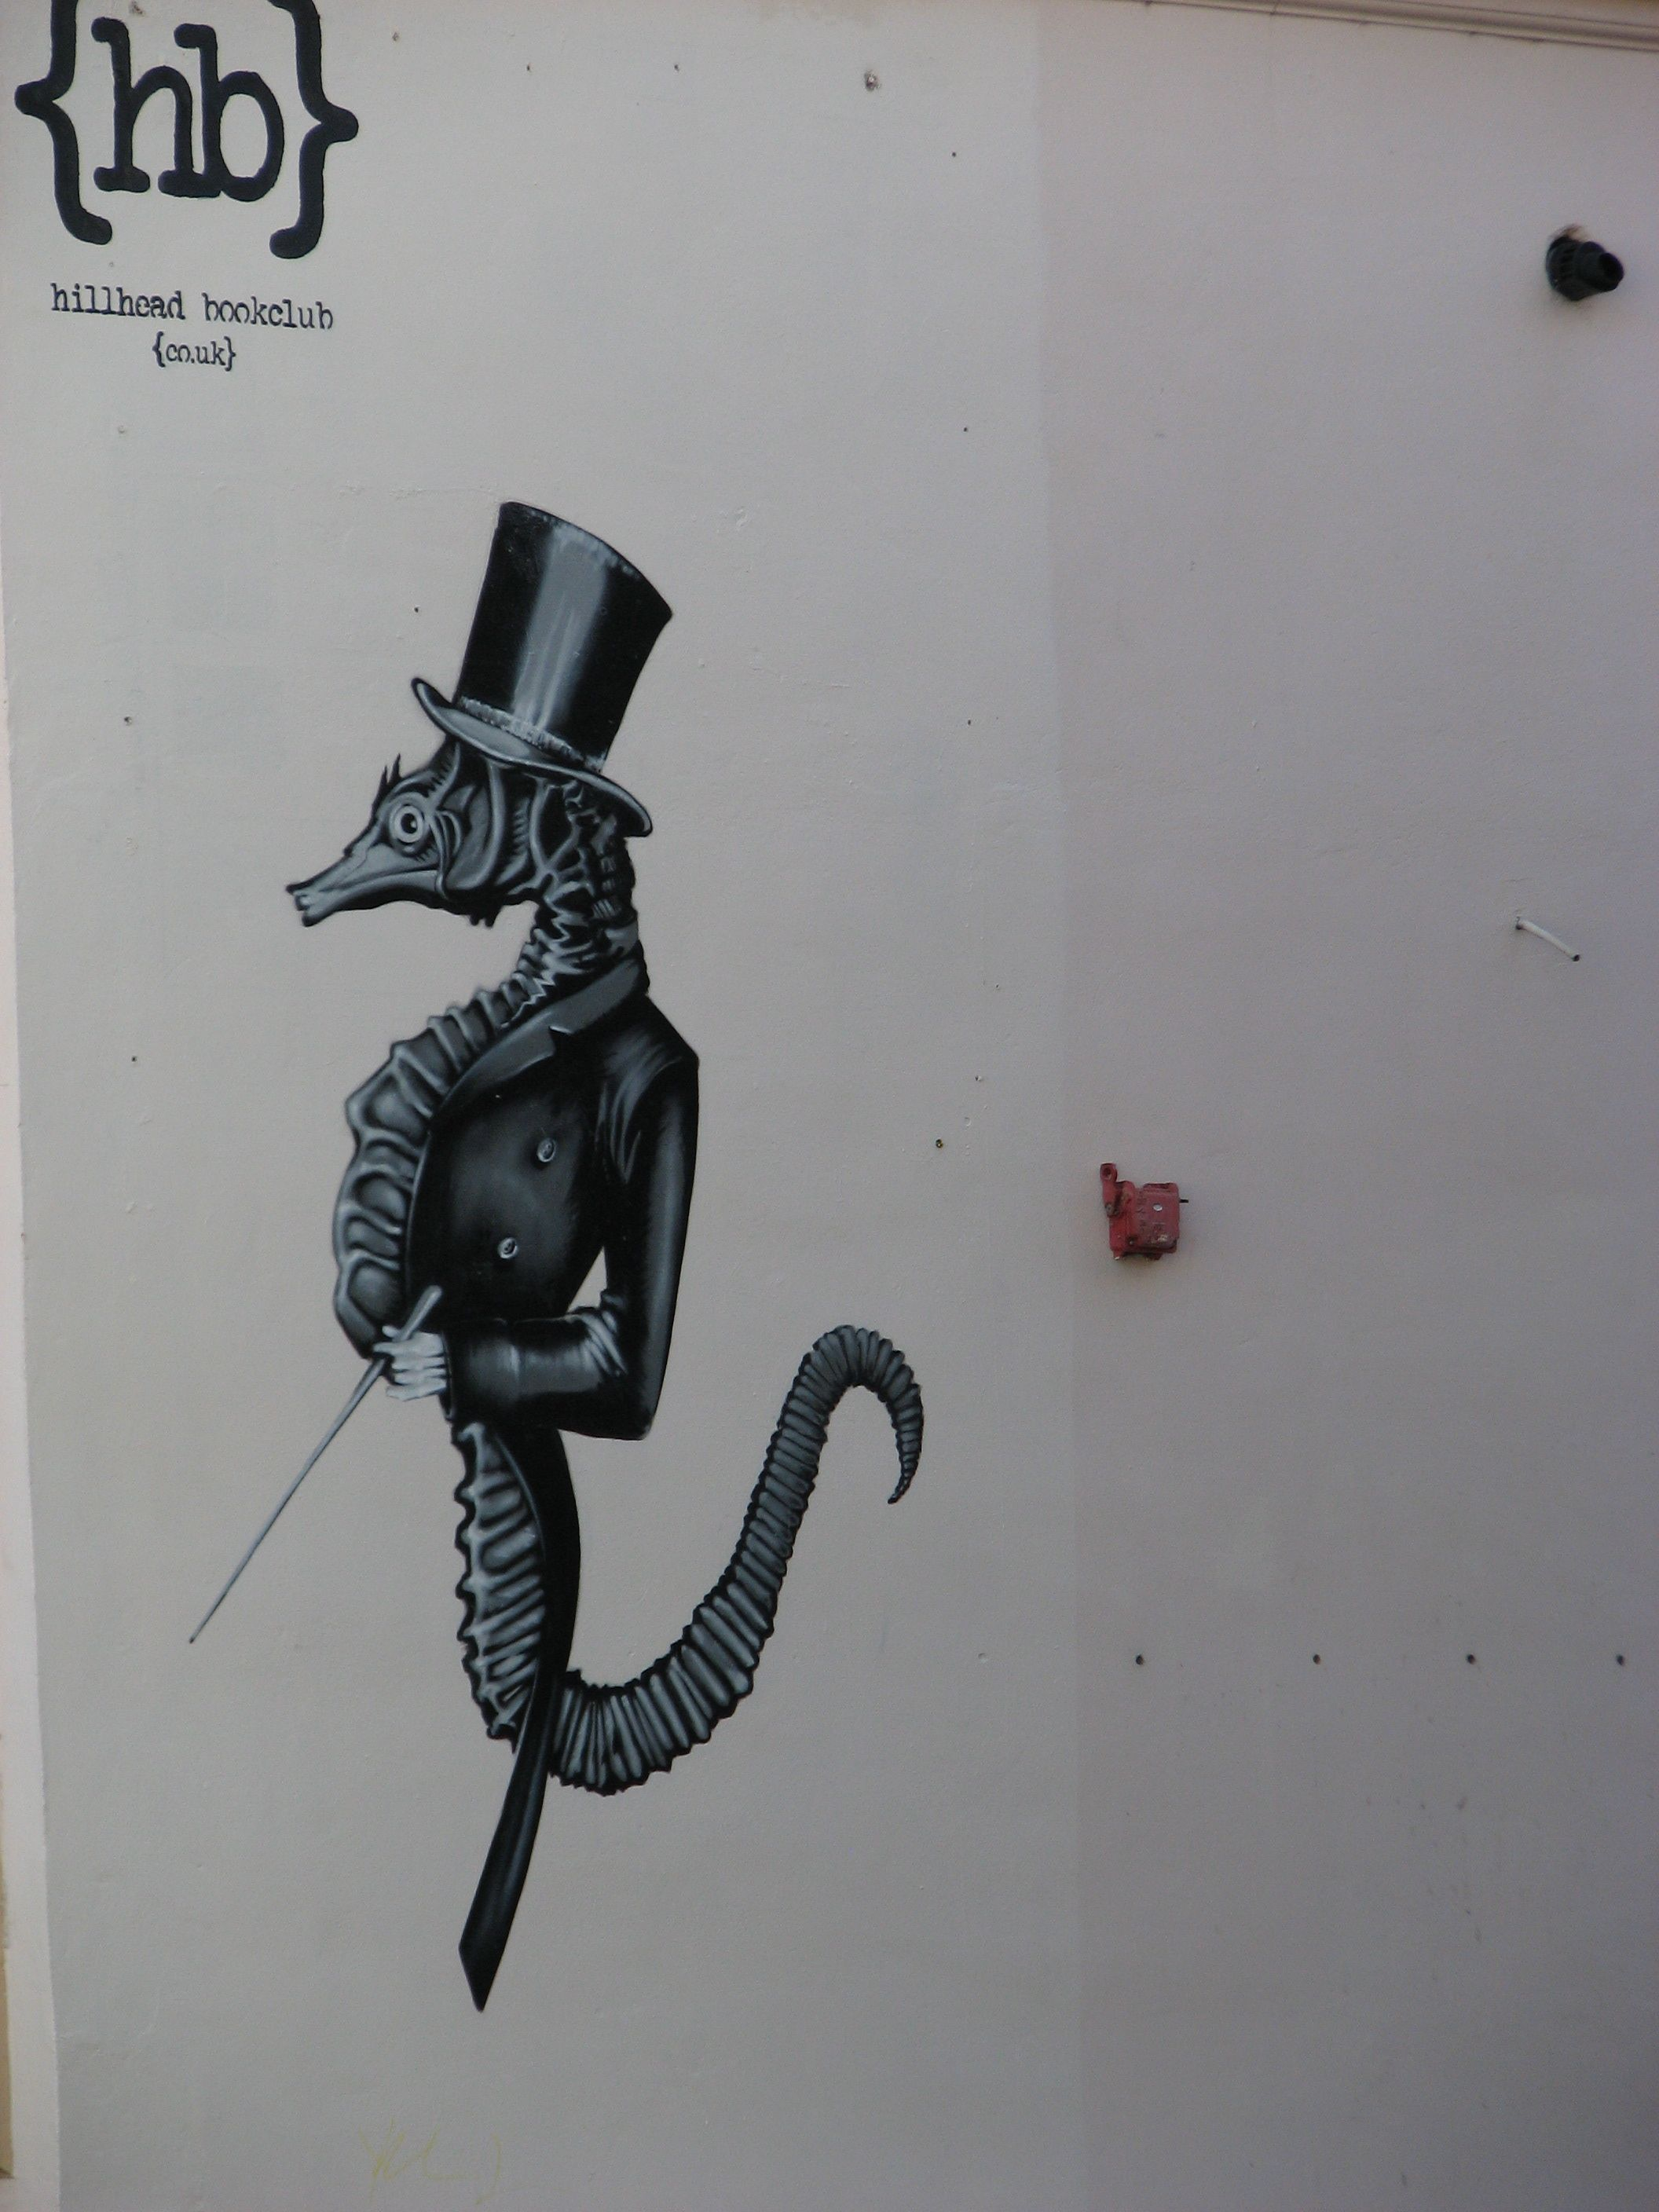
\includegraphics[scale=0.10]{hb1}
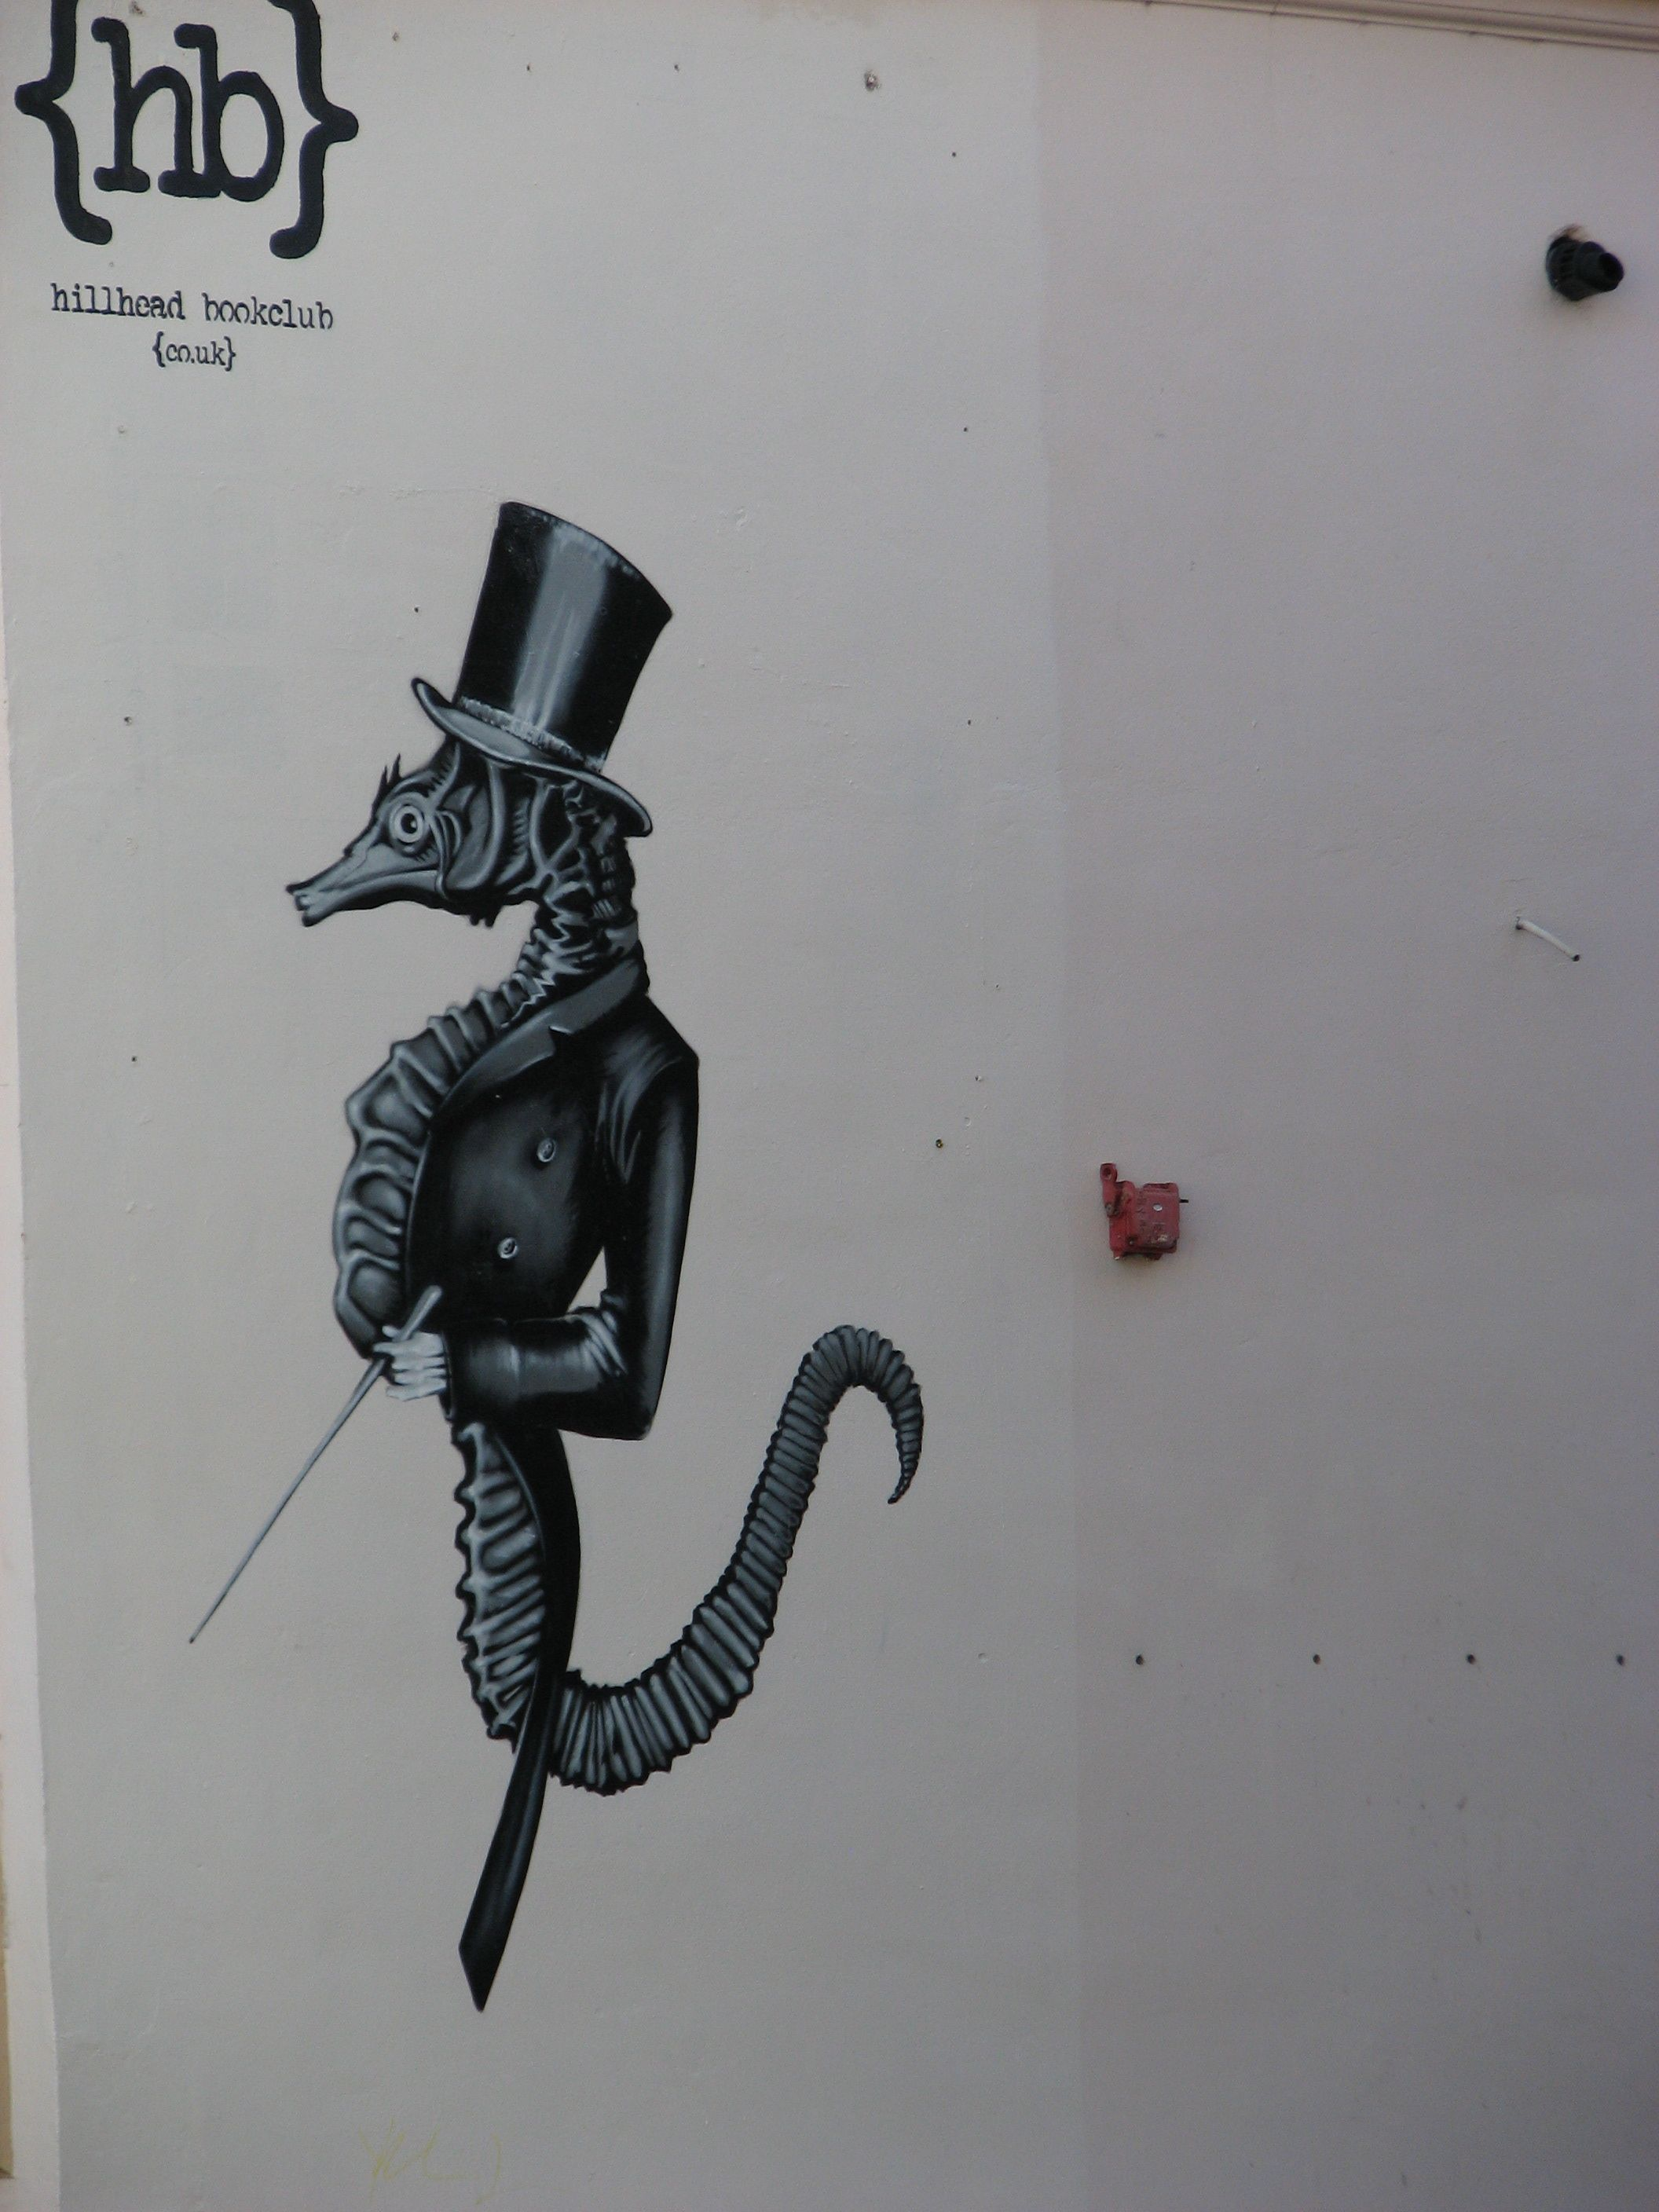
\includegraphics[scale=0.10]{hb1}
\caption{\emph{The images above show that there are no obvious differences between an unaltered image and the same image with data embedded in it using open source steganographic software called Stepic \cite{stepnic}. The image on the right contains the following text embedded using steganography : ``Thoughts, words, and deeds, the statute blames with reason;  But surely dreams were ne'er indicted treason \cite{burns}"}}
\label{fig:stegexample}
\end{figure} 
%Steg image
Colour images, for example, can use anywhere between 4 to 8 bits of data to represent one colour value of a pixel (either red, green or blue). A change to a single bit for each colour would still ensure that the image resembled the original \emph{See: Figure \ref{fig:stegexample}}.
Image steganography is perhaps the most popular used form of digital steganography as a large number of freely available tools that allow one to embed data in images are easily available. These tools, described in more detail in Chapter \ref{ch:litsurvey} allow for embedding data in almost any image format. Some of these tools also provide encryption using a password derived key to provide an additional layer of security to the embedded data. The hidden message can then be recovered by the recipient with a suitable decoding tool and the correct password or decryption key. This makes image steganography a viable medium for covert communication.  
Another interesting use of image steganography is for the purposes of copyright enforcement  \cite{kundur2002digital}. By using digital watermarks that contain copyright information,  it is possible to uniquely identify an image even after it has  been modified. These ``marks'' can be read by specialised software which can determine the original source of the image. 
\par The use of image steganography as a covert communication channel on the internet has always been a contentious topic and a source for much speculation. Analysis of a terrorist user manual, the Technical Mujahid \cite{alfajr}, by the United States Central Intelligence Agency (CIA) mentioned chapters in that outline various concealment techniques utilising image steganography. The manual describes the use of steganography as an additional layer of security for encrypted data. It's however, difficult to ascertain whether these techniques are in use in the wild. An argument for the limited use of steganography would be that steganography is an approach that relies on security through obscurity. Security through obscurity implies the use of a secret, but insecure, method of protecting a resource. An example of this would be hiding one's room keys under the doormat in the hope that a thief would never find it there. In 2000, Provos and Honeyman \cite{provos2001detecting}  carried out an analysis of images available on eBay for steganographic content.  They argue that either there isn't  significant use of steganography on the internet or that the steganographic techniques used are undetectable by the methods used by them. They also concede that it might be possible that encryption might have been used on the data embedded in the images and that they were unable to decrypt it. Their analysis is based on a fairly large (2 million) image dataset acquired from eBay.   More recent news reports  \cite{spies2010} suggest that members of a Russian spy ring arrested in the United States in 2010 used steganography to communicate with each other. Reports speculate that these individuals posted images with steganographic content on public image hosting sites with sensitive data embedded in them. The news reports, however, did not provide any technical details regarding the steganography methods used. This project attempts to revisit the seminal work conducted by Provos \emph{et al} to try and establish real world usage of steganography.

It would be trivial to prove the \emph{existence} of steganography if one were provided the unaltered host image along with the image carrying the steganographic payload. By calculating the binary difference of the steganographic image from the unaltered image, one could easily discover the payload embedded in the image. However, this is an unrealistic expectation as the steganographic host medium will be less likely to be found along with the altered copy. Hence it is necessary to user other means for the steganalysis of images that do not require the original host image for comparison.


\section{Terminology}
The following terms are used throughout the document to refer to various aspects of steganography. 
\begin{itemize}
\item{\emph{Steganogram:}} An \emph{portmanteau} of steganography and telegram, this is used to refer to an image containing steganographic content. The content could be text, images or audio. In this report, a steganogram is used to refer to an image containing hidden text.
\item{\emph{Stegnanalysis:}} The process of testing a digital artifact for embedded steganographic data. This analysis may be carried out either using statistical measures or by matching the contents of the digital artifacts against a database of known steganographic signatures.
\item{\emph{Cover medium:}} Any digital medium used as a host for hiding data. Throughout this document, the cover medium is used to refer to digital imagery.
\end{itemize}


%\chapter{Literature Survey}
\label{ch:litsurvey}
In this section, prior work in the field of image steganography and steganalysis are explored. This chapter is divided into four sections. The first section discusses popular steganographic implementations that are to be detected using the experimental set-up. The second section describes theoretical work in analysis of these steganographic schemes. Software tools that implement various types of image steganography are discussed in the third section. In the final section of this chapter a number of freely available software packages that implement steganography are evaluated.
\section{Approaches to Image Steganography}
\label{sec:overview}
A large amount of literature exists on different methods to encode data in images. Early work in this area explore secure digital watermarking techniques for copyright enforcement which led to the creation of robust watermarking algorithms that were resilient to image manipulation. The use of similar techniques for secret communication using digital images followed thereafter. Freely available steganographic tools implement one or more of the following algorithms for embedding data in images. The data need not be restricted to text, it is possible to embed any other digital format into images. 
\begin{itemize}
\item Least Significant Bit image steganography:  LSB encoding is perhaps the most simple form of steganography. In this form of steganography, the image to be used can be represented as an array of RGB tuples with each colour value represented as a binary string. If the image is a 24 bit colour image, each colour value is represented by 8 bits as shown in \ref{eq:lsb}. The message to be encoded is usually compressed and encoded as a binary string. A simple algorithm would now begin encoding the data into the image starting from the first colour value representation and moving on until it has finished encoding the entire message. 
\begin{equation}
\label{eq:lsb}
\begin{split}
\text{\emph{Bits from image}}
\\
10110011\ 10001101\ 11111011 \\
10111000\ 10010100\ 01110111 \\
\\
\text{\emph{Bits to be encoded}}
\\
101100\\
\\
\text{\emph{Result, modified bits are shown in bold}}
\\
10110011\ 1000110\mathbf{0}\ 11111011 \\
1011100\mathbf{1}\ 10010100\ 0111011\mathbf{0} \\
\end{split}
\end{equation}
Variants of the LSB steganography algorithm may use random bits of the host image which can be dervied from a secret key. Visual changes caused to the image are minimal for 16bit/24bit colour images. If the colour depth is lower, a substantially large message (< 25\%) would cause degradation in image quality. 
\item Frequency Domain Encoding: This is a slightly more sophisticated steganographic technique and is implemented in a number of tools like JSteg \cite{jsteg}. This scheme uses colour frequencies of the host image to hide data. The frequency distribution can be transformed into a ring structure by using a 2D Fast Fourier Transform (FFT). The FFT function, when applied to the image frequency distribution produces a ring like structure with the lower frequencies represented at the centre and the higher frequencies towards the edges. By converting a digital image into its constituent frequency distribution and subsequently using a 2D FFT function, it is possible to utilise the mid-range frequencies to encode data. The host image containing the steganographic message is retrieved using an inverse FFT that returns the image. Both LSB encoding and Frequency Domain Encoding require images that are approximately 3 times larger than the message to be encoded. Frequency Domain Encoding provides better protection against the discovery of the secret message when compared with Least Significant Bit encoding and is only marginally affected by file compression. 
\item BPCS encoding : Bit-Plane Complexity Segmentation Based Embedding is a relatively new and potentially more effective way of data hiding.  A digital image can be segmented into a number of bitplanes of increasing complexity \cite{kawaguchi1998concept}. This segmentation divides the image into planes in such a way that each plane contributes some amount of detail to an image. The higher order planes contain the most detail and represent the features available in the image. The lower order planes contribute very little and appear as noise when viewed on their own.  For an image of size $n$ it is possible to use as much as $\frac{n}{2}$ of the image for hiding data provided that the image is sufficiently complex. For simpler images, any alteration to lower order bit planes that constitute the image would be readily evident.
\item Image File Padding: This method of steganography does not require modifications to the colours of the image directly. Instead it relies on the fact that it is possible to pad an image towards the end with the secret. This is also not a very reliable scheme as padding a large amount of text into a relatively small image would cause the image file to be corrupted. It would, however, work reasonably well for small sized textual data (< 10\% of image size).
\end{itemize}
\section{Previous Work in Steganalysis}
\label{sec:theory}
Pfitzmann and Westfield \cite{westfeld2000attacks} describe two methods for analysing images for steganographic content. The first method is the use of visual techniques to identify whether an image could contain steganographic content.  This is done by first extracting the potential message bits (\emph{i.e.} bits of the image that may have been used for hiding data). The other bits of the image that are non steganographic are removed and only potential message bits are illustrated using black and white. This allows an observer to see that the image may contain data.
\begin{figure}[h!]
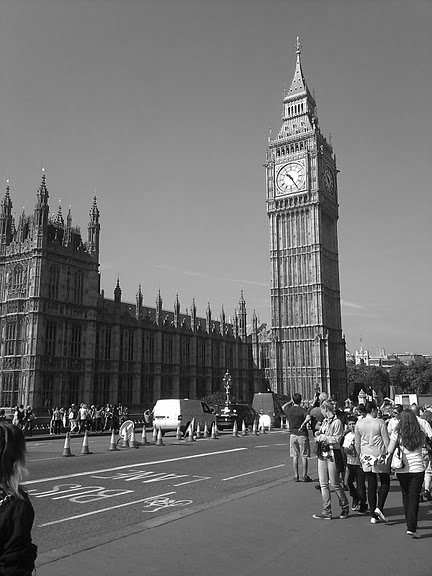
\includegraphics[scale=0.10]{visual1}
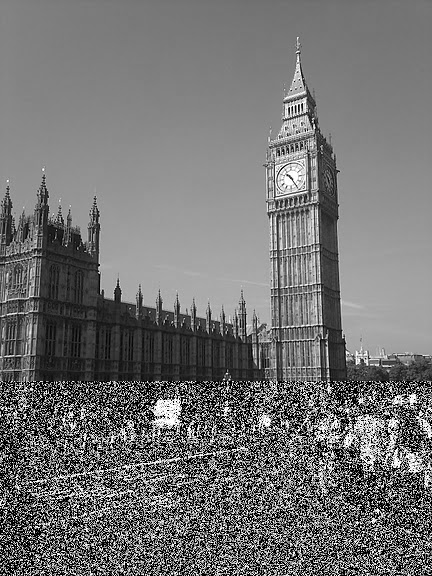
\includegraphics[scale=0.10]{visual2}
\caption{\emph{Blah}}
\label{fig:visualattacks}
\end{figure} 

\par The second method utilises the $\chi^{2}$ statistical test to determine if the image contains steganographic content. In this method,  the theoretical expected frequency distribution of pixels in an image is compared with the actual frequency distribution of the pixels in the steganographic image. A deviation between these values indicates the presence of a steganographic message. This is possible as the tools used for creating the steganographic image incorrectly assume that the Least Significant Bits are random and can be overwritten to hide message. The authors claim that statistical tests provide a much higher accuracy than visual attacks and should be used when possible. 
\par Building on the works of Pfitzmann et al  \cite{westfeld2000attacks}, Fridrich and Goljan \cite{fridrich2002practical} present a collection of qualitative methods for practical steganalysis. The authors extend the statistical analysis described by both Pfitzmann and Provos to include the spatial arrangement of pixels in a steganographic image referred to as ``Dual Statistical attacks''.  
\par The JPEG compatibility attack described by Goljan et al relies on finding non compatible JPEG artefacts in images. The image to be analysed is divided into  8x8 pixel blocks and the algorithm attempts to locate blocks that would not ordinarily be produced by the JPEG compression algorithm.
\par A universal, ``meta'' steganalysis approach from Farid  \cite{farid2002detecting} is also described by the author, which attempts to detect the presence of steganography rather than being a targeted approach towards a specific steganographic algorithm.  This approach utilises higher order statistical modelling that provides a generic approach to detect the presence of steganographic content in images. Farid's experimental setup consists of three types of support vector machines (SVMs). A support vector machine is a data classifier with a very high degree of accuracy \cite{noble2006support}. The kernel parameters for the support vector machine were tuned as to provide a very low (1.0\%) false positive rate. They were then trained with a library of GIF, JPEG and TIFF images. The trained SVMs were used to classify a large number of mixed (steganographic and non steganographic) images. It was discovered that with a low false positive rate, a non-linear SVM was able to accurately classify 90.2\% of steganographic images of size $160\times160$ pixels correctly with a false negative rate of 9.8\%.
An exhaustive study carried out in 2001 by Provos and Honeyman \cite{provos2001detecting} analysed over 2 million images publicly available from eBay auctions using a similar method. Images that were classified as being suspicious were subjected to a dictionary attack in order to attempt recovery of the message.
\par Their results did not find any significant use of steganography in images that were posted as part of the auctions. However they do not discount the possibility that the images they analysed were using steganographic techniques that were not not detectable by the methods employed by them.
\par For the few thousand images that were discovered to have been marked as suspicious by their setup, it was not possible to recover any of the messages embedded in them.  They speculate that it could have been due the use of a strong password to encrypt the message stored in the images.

\section{Image Steganography Tools}
\label{sec:tools}
In this section an overview of popular steganographic tools is presented. It was found that while a number of tools are available for steganography, many of them share similar algorithms to encode data in digital files.  The tools are evaluated on the basis of their availability, the operating system platforms they support and the algorithms implemented by them. Non free tools were not evaluated as part of the project. 
\subsection{EzStego}
EzStego \cite{ezstego} is a free steganographic tool created by Romana Machado  implemented in Java and is available for the most common operating systems (Linux,Windows, MacOS). The software appears to be no longer maintained but copies of it are mirrored in other locations of the web. The steganograms produced by EzStego have been extensively studied by a number of authors  \cite{westfeld2000attacks, farid2002detecting}. It is most susceptible to the visual attack as it relies of Least Significant Bit encoding (LSB) to hide data in a GIF file. 
\subsection{S-Tools}
S-Tools \cite{stools} are a collection of steganographic tools that allow for data hiding in a number of digital file formats. Supported formats include WAV, GIF and BMP files. It is not possible to use a JPEG file as a medium for steganographic data using this software.  S-Tools also allows the user to choose between DES, Triple DES, IDEA and MDC encryption algorithms. In order to recover data from S-Tools created steganograms,  the user is required to know the passphrase that was used as the key to encrypt the data and the encryption algorithm used.  S-Tools is available for Windows and UNIX like operating systems.
\subsection{JSteg} 
JSteg \cite{jsteg} is a steganographic tool that allows a user to embed messages in JPEG files, the message size is limited to roughly 12\% of the image size. It has been extensively studied by a number of authors including Westfeld and Goljan. The image medium used is JPEG, which is a lossy image compression algorithm. Owing to this images containing data encoded with JSteg are immune to traditional visual attacks unlike EzStego, which requires an uncompressed Bitmap image as the medium. Due to the use of JPEG as an the medium, it is not possible to reliably isolate data that is encoded in the least significant bit field and prove the existence of steganography. Steganograms produced by JSteg are, however, still vulnerable to statistical attacks. JSteg is written in C and is available for Windows and UNIX like operating systems.
\subsection{JPHide and Seek}
JPHide and Seek \cite{jphide} was written by Alan Latham and it is exclusively designed to hide data in JPEG images. It's primary design goal is providing plausible deniability \emph{i.e.} it should be difficult or impossible to prove that a particular image contains steganographic data. This goal is acheived if the message length is less than 15\% of the size of the image and the image contains significant detail (\emph{e.g.} a picture of a forest with a river). Separate versions for Windows and Linux are available.
 \subsection{F5}
 The F5 algorithm \cite{westfeld2001f5} was created by Westfeld to provide a steganographic solution that was resilient to both visual and statistical attacks. This is made possible by the design of the F5 algorithm that uses matrix encoding for data and uses permutation techniques to distribute the data throughout the steganographic medium. Unlike LSB based steganography software like JSteg and S-Tools, F5 encodes data by manipulating the DCT coefficients in a JPEG image. 
 \subsection{StegMark}
 StegMark \cite{stegmark} is a commercial software product developed by DataMark Technologies. It is not strictly designed for steganographic communication; instead this software implements digital watermarking using steganography. Digital watermarking can be used to enforce digital content ownership and prevent plagiarism of images or other digital media. It can, however, be used to communicate covertly as it provides an SDK for creating steganography tools. StegMark is available for Windows as a C++ SDK.
 \subsection{Stepic \& ESFS}
 Stepic \cite{stepnic} is a relatively new steganography tool written by Lenny Domnitser in Python. The steganography implementation appears to be pedagogical as it only provides data hiding by using LSB encoding. Another project, the Encrypted Steganographic Filesystem (ESFS) \cite{esfs}, has adapted Stepic to provide a File System in User Space (FUSE) based filesystem for Linux. StegFS also provides an additional security by encrypting the data using AES with a 256 bit key. It is a proof of concept implementation and the author claims that the performance is relatively poor. Stepic is available as open source software for both Windows and UNIX like operating systems while ESFS requires Linux and Python with the cryptographic toolkit (pycrypto) installed.
 \subsection{Digital Picture Envelope}
 Digital Picture Envelope is the result of research \cite{kawaguchi1998concept} in the area of Bit Plane Complexity Steganography(BPCS). This method of steganography is radically different from the other implementations that rely on LSB encoding to hide data. The Digital Picture Envelope converts the host image into a number of bit planes, each plane constitutes part of the image. The most complex planes can be used as information carriers as changes to it cannot be perceived by the human eye.  An added advantage is that unlike other steganographic mechanisms, BPCS \emph{alters} the actual image instead of appending to it thereby ensuring that the steganogram is the same size as the original image. Additionally, up to 50\% of the image can be used to store the data. Digital Picture Envelope is available in binary format for Windows systems only. 
 
\section{Image Steganalysis Tools}
\label{sec:steganalysistools}
In this section we discuss a number of tools that provide steganalysis features. There are very few free tools that implement all steganalysis attacks.Proprietary tools rely heavily on image hashsets and other proprietary detection methods that are not disclosed. For the purpose of this project it wasnecessary to identify a set of tools that will provide a universal system for steganalysis \emph{i.e.} the tools should be able to prove the existence of steganography in a given image. Some of the tools that implement steganalysis are:
\begin{itemize}
\item Outguess : Outguess \cite{outguess} ships as a package that provides steganography tools as well steganalysis tools. It implements custom detection routines for popular steganography algorithms like JSteg, F5 and JPHide. It also provides the command line tools stegdetect and stegbreak, the former implements steganography detection while the latter provides a tool that attempts to extract data from a steganogram using brute force and dictionary attack methods. It is available as open source software with source and binaries for all platforms. 
\item Virtual Steganography Laboratory: VSL \cite{wegrzyn2009} is provided as an open source steganography and steganalysis Java software package. It implements F5 \cite{westfeld2001f5}, Karhunen-Loeve Transform \cite{stanescu2007digital} and Least Significant Bit steganography.
\item Gargoyle : Gargoyle \cite{gargoyle} is a commercial malware removal product that ships with a proprietary database of hashsets. These hashsets provide a method of identifying steganographic content by checking for ``signatures'' left by steganographic software. The software package is available for Windows and is designed for forensic investigators.
\item EnCase : Another commercial software product \cite{encase} that provides various  computer forensic features. It has features that allow for steganographic detection. Encase runs on Windows and employes signature based detection to check for the presence of steganography.
\item AccessData Forensic Toolkit :  This commercial tool allows for the identification of steganography based on proprietary hashsets \cite{ftk}. Like Gargoyle and Encase, it can only identify the presence of steganography in files by means of hash analysis. It is limited to identify a finite number of specific steganography algorithms. 
 
\end{itemize}
The availability of free image steganalysis tools is limited as compared to the numerous options available for image steganography. A few steganography suites, like Outguess \cite{outguess} provide a combined steganography/steganalysis software suite. Commercially available tools like Encase, provide steganalysis as part of a digital forensics toolkit.  


%\chapter{Experimental Design}
\label{ch:dev}
Based on the evaluation of tools and previous work in the area of
steganalysis, an experimental setup is described to test a random sample
of images for steganography. In this section I propose a hypothesis that
is to be tested using the experimental setup. The images used as part of
the study were obtained from Gumtree, Ebay and Craigslist with the
majority of the images obtained from Gumtree. Ebay and Craigslist appear
to employ throttling mechanisms that prevented the spiders from
gathering a large number of images.
\section{Hypothesis}
\label{sec:hypothesis}
In Section \ref{sec:practical}, we discussed the work of Provos and
Honeyman in the area of practical steganalysis. It is proposed to test
the following hypothesis:
\par
\emph{The use of image steganography as a means of covert communication
is non existent as it is possible to reliably identify images containing
data embedded with popular steganographic tools with a reasonably high
degree of accuracy. It follows that primary motive for the use of steganography as a
means of secretive communication in plain sight is effectively nullified
with the availability of detection tools like stegdetect}. 

Additionally, the experiment is subject to the following constraints:
\begin{itemize}
\item{Image Type}: The experiment is focused on analysis JPEG images
gathered from the internet. All other image types are excluded and
ignored by the crawler.
\item{Image Size}: All analysed images are larger than 100x100 pixels in
size and have a colour depth of 24 bits. This threshold has been chosen since it 
is assumed that smaller image sizes would provide very little bandwidth
for steganographic content.
\end{itemize}
\par  Previous experiments that have successfully identified images containing steganographic have done so under lab conditions with strictly defined parameters for image size, colour depth and resolution. Images available online vastly differ in size, resolution and colour depth. Additionally, they might be created using different versions or implementations of the same compression algorithm. 

\section{Control}
\label{sec:control}
It was required to have a control data set of ``clean'' images to
determine the number of false positives determined by
\texttt{stegdetect} as well as to evaluate the performance of stegdetect. I used a set of personal JPEG images collected from
a Canon S3IS camera over the last few years. The images were scanned
using \texttt{stegdetect} in their original resolution (average 5
Megapixels) as well as after
being cropped to a size of 500x500 pixels.



\section{System Architecture}
\label{sec:sysarch}
The system architecture is as shown in Figure \ref{fig:architecture}.
The crawler is implemented as a set of spiders for each website to be
crawled. In the initial design, each spider started at the root of the
website to be crawled and discovered links for further crawling. Each
discovered link was then recursively crawled and any images discovered
were downloaded using the \texttt{ImagePipeline}.

However, the performance obtained from this setup was not satisfactory
and an alternate approach to downloading images was devised. Instead of
recursively crawling the domain, a copy of the website's entire sitemap was
obtained. Conventionally, most websites provide a gzipped XML file at
the root of the domain to allow Google and other search engines to
effectively crawl the website. The sitemap file describes the location
of each URL available on the site using the \texttt{url} tag. These URLs
can be extracted using a simple XML parser.

Once the URLs from each site was extracted using an XML parser over the
sitemap, they were added to a plain text file. A simple bash script was
created to instantiate the spiders with a part of the URL list file.
This was done to avoid creating a large URL dictionary that would
severely degrade performance of the crawler. By using prepared regular expression to precisely define the
location of the images on each HTML file parsed, a substantial increase in performance was
obtained.

Upon parsing a single HTML file, any images found on it are passed
on to the \texttt{ImagePipeline} class as well as the
\texttt{DbPipeline} class. The latter creates an asynchronous SQL query
to store the metadata associated with the image. The database
schema is defined in detail in Appendix \ref{appendix:schema}.

If an image obtained from the \texttt{ImagePipeline} is not of the appropriate size, it is discarded from the
queue of images to be downloaded. All other images in the queue are
downloaded asynchronously after they have been added to it. The
components of the setup are described in more detail in the following
subsections


\begin{figure}[h!]
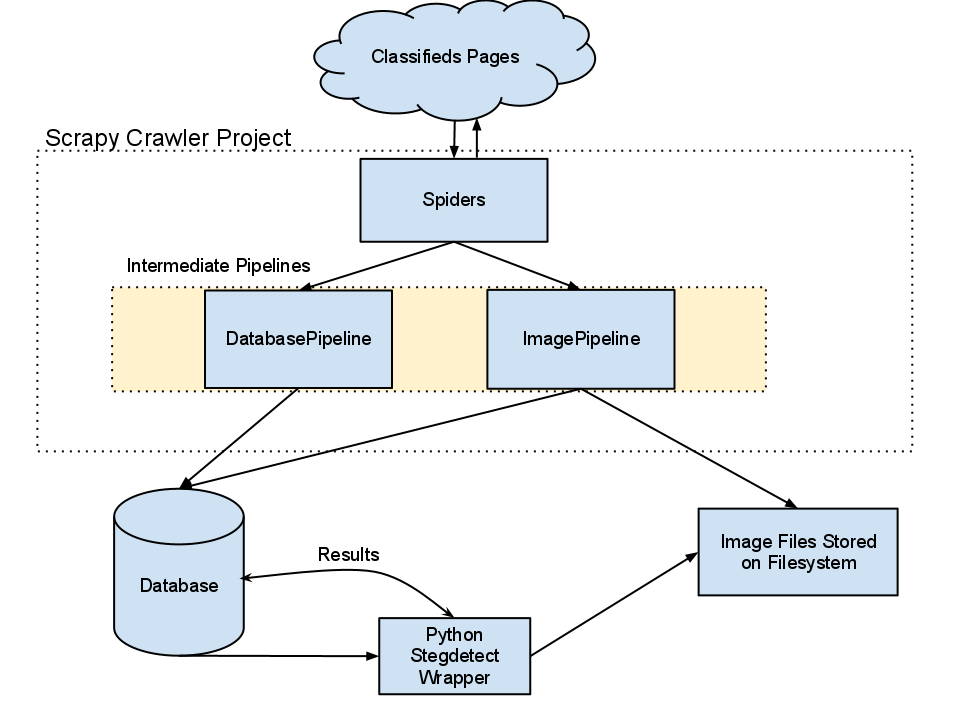
\includegraphics[scale=0.5]{ArchDiagThesis}
\caption{\emph{An overview of the system architecture}}
\label{fig:architecture}
\end{figure} 
%Describe the design
%Describe how all the components fit in together
%Describe how it all differs from the proposal design

\subsection {Web Scraper}
\label{sec:scraper}
%What is a scraper?
%What does it consist of?
%Why do you need it for these project?
%Why did you choose scrapy?
%How does it work?
A scraper allows an application to retrieve and store specific items from a web page. Any part of the HTML Document Object Model (DOM) can be selected and extracted for further processing, a process known as scraping. Most crawlers consist of two main components, a web crawler that allows it to collect a large number of pages quickly and the actual scraping module that allows for the extraction of relevant content. A large number of free and open source projects are available that provide both kinds of functionality. For this project, scrapy was used as the basis for the web scraper based on previous evaluations and it's excellent database connectivity and image handling options.
\par Scrapy is a python web framework that can be used to build web crawlers/scrapers. It was designed primarily for programmatically accessing websites that do not explicitly provide an Application Programming Interface (API). Scrapy does not provide an implementation of a specific scraper, it provides a number of classes that can be used to create a custom scraper. A scrapy project consists of one or more spiders and pipelines that determine what happens once an item has been downloaded. The crawler component was created by extending scrapy's \texttt{BaseSpider} class. The \texttt{BaseSpider} class requires the implementation of a \texttt{parse()} method that determines the action to be taken when an HTML page is encountered. The \texttt{parse()} method is called on every invocation of the spider. Relevant elements in the HTML page are selected using HTML XPath queries. In this implementation, the \texttt{parse()} method yields subsequent HTTP requests that the crawler needs to make subsequently using the URLs found on the page. An \texttt{Item} class is also created for each JPEG image found on the page. These images are then added to a python dictionary and returned to the \texttt{ImagePipeline} middleware.
\par The \texttt{ImagePipeline} middleware is responsible for the scheduling and downloading of image files. For each dictionary of items returned by the crawler, the pipeline enqueues the URLs of the images found and downloads them asynchronously. Saved images are named according to the MD5 hash of their content so that they can be uniquely identified at a later stage. After building a suitably large collection of images, steganalysis was carried out on each of the images as described in the next section.
\subsection {Steganalysis}
\label{sec:stegtool}
Steganalysis on the downloaded images is carried out using \texttt{stegdetect} which is part of Provos' Outguess suite of steganography tools. \texttt{stegdetect} provides detection features for six different kinds of JPEG steganographic algorithms namely jsteg, outguess, jphide, invisible secrets, F5 and text appending. For each steganographic algorithm detected by \texttt{stegdetect} it provides a confidence rating between one to three stars. It also provides a parameter for tuning the sensitivity of the scanner. The sensitivity can be specified as a floating point number, which would cause the confidence rating to be multiplied by it. For this project, \texttt{stegdetect} was used only to try and detect algorithms known to it although stegdetect allows for feature extraction that can be used to detect unknown algorithms. The detection was carried out using four different sensitivity settings (0.25, 0.5, 0.75 and 1) in order to minimize false positives.
\par A custom python script was created to wrap \texttt{stegdetect} and generate output in a way suitable for database storage. Finally, the data obtained was saved in a database for further analysis.
\subsection{Database Structure}
\label{sec:dbstructure}
The initial database chosen for the project was sqlite as the application had modest data requirements. However, sqlite ended up causing a large amount of data corruption and was the source of thread concurrency errors. The data was then migrated to a MySQL database and the code was modified accordingly.A single data table stores details of the downloaded images which are generated by the middleware after each image has been downloaded. 
\par Each image is uniquely identified in the database by an auto incrementing primary key. Steganalysis is carried out by obtaining the path of each image from the database and running stegdetect on them. The results of the steganalysis are stored in an analysis table which uniquely identifies each result by an autoincrementing primary key and references the primary key of the image from the data table.
\par  All access to the database is through a connection pool that maintains 4 connections to the MySQL database. This was implemented by extending a class from the python twisted library called the Asynchronous Database Access API (twisted.enterprise.adbapi). Adbapi provides a non blocking interface to the database and vastly improves random read/write access when compared to standard database APIs like the standard python MySQLdb API. The adbapi class was modified to handle reconnections to the database as it was discovered that the provided MySQL database frequently dropped connections between transactions. 
\section{Summary}
\label{sec:devsummary}
This chapter describes the experimental setup to be used as well the
hypothesis that is to be tested. Detailed instructions to replicate this
setup can be found in Appendix \ref{appendix:setup}. In the next
chapter, the setup is evaluated and the results obtained from it are
analysed.


%\chapter{Evaluation}
\label{ch:evaluation}


%\chapter{Conclusion}
\label{ch:conclusion}

%\bibliographystyle{plain}
%\bibliography{thesis}
\end{document}


